\documentclass[onecolumn]{IEEEtran}
\usepackage[numbers]{natbib}
\usepackage{amsmath}
\usepackage{float}
\usepackage{caption}
\usepackage{graphicx}
\usepackage{enumitem}
\usepackage{url}
\title{\textbf{ActiWate: Adaptive and Design-agnostic Active Watermarking for IP Ownership in Modern SoCs}}
\author{{\large Arpit Kumar}\\ Department of Computer Science,IIT Bhilai\\ 12340350 \\ {{arpitk@iitbhilai.ac.in}}}
\date{}

\begin{document}
\maketitle
\begin{abstract}
\textbf{	Watermarking offers a viable solution to combat IP piracy
	and illegal re-use. However, watermarking verification techniques rely
	heavily on manual testing by verification engineers and ignore the
	possibility of having a rogue SoC design house. To automate the
	watermarking-based verification process and to be against wider attacks
	(e.g., rogue design house), this paper presents \textit{ActiWate}, which conducts
	automatic self-verification by communicating with various peripherals
	within the SoC. Showing its resilience against removal and spoofing
	attacks, \textit{ActiWate} is architectured to be an IP/SoC-agnostic watermarking
	and our experiments demonstrate its versatility by implementing it on
	multiple RISC-V SoCs with different components/peripherals.\\
	Index Terms—Watermarking, IP Authentication, Hardware Security}
\end{abstract}

\section{INTRODUCTION}
\label{sec1}
System-on-Chips (SoCs) are becoming ever-increasingly complex
as they support more functionalities for addressing the demand for
more advanced technologies. In such circumstances and with tight
time-to-market, SoC design teams commonly license pre-designed
intellectual property (IP) cores as soft (RTLs), hard (GDSIIs), or firm
(netlists) IPs. Additionally, to maintain cutting-edge semiconductor
fabrication more affordable, fabless semiconductor companies outsource post-silicon stages, i.e., fabrication, testing, and packaging, to
offshore foundries. With the combination of re-use and globalization,
we witnessed boosted growth, lowered costs, and cut time-to-market
in the semiconductor industry. However, as the IP rights owner may
provide the SoC integrator (and foundry) with the entire specification,
the IP owners are no longer the sole proprietor of content. This
IP procurement business risks violating the original license terms
and misappropriating the design. In such a process, several security
vulnerabilities arise as a result of the untrusted parties within the
supply chain, e.g., IP theft, counterfeiting, reverse engineering (RE),
and integrated circuits (ICs) overproduction \cite{a}. Since IP owners have
very little control over the illicit use of their IP, identifying IP cores
within suspect designs is imperative.

Numerous studies have investigated various techniques to prevent
IP cores from being exploited illegally, e.g., IP encryption, active metering, logic locking, watermarking, etc. \cite{b}-\cite{Anandakumar2022}. Widely used through
the last two decades, Watermarking embeds a unique signature into
an IP core (building the watermarked IP) in a way that does not alter
its original functionality. When the chip is ready (fabricated), the
IP owner can retain it and extract its signature using the activation
parameters they created to prove the legitimate use of their IP core
in the SoC by comparing it with the initially embedded signature.
Watermarking must be easy to embed/verify and not burdened with
high overhead and attacks \cite{Chang2016}. Although other countermeasures like
logic locking can prevent IP infringement, piracy, and overproduction,
watermarking primarily focuses on verifying the legality of IP reuse, and with several copyright violation incidents in the past two
decades\textsuperscript{1}
, having unique identifier per each is a must for IP ownership
proof.

Several watermarking methods have been introduced in the literature, which can be divided into five major categories \cite{Anandakumar2022},\cite{Das2022}-\cite{Kibria2022}:
(1) Constraint, (2) Digital signal processing (DSP), (3) Finite state
machines (FSM), (4) Test structures, and (5) Side-channels based
watermarking. For a watermarked IP (any watermarking technique),
when a rogue SoC integrator pirates the IP without any contract with
the IP owner, they restrict (block) direct access to the IP. In this
case, only the inputs/outputs (I/O) of the IC (+ test infrastructure)
are available for proving ownership of the IP (not the I/O of the
IP), enabling the rogue integrator to use the IP illegally in different
ICs. Existing watermarking techniques do not explicitly address the
extraction of watermarks in such cases. An IP owner may extract the
watermarking signature if the signature is side-channel based \cite{Ziener2006}.
However, techniques like FSM and test-based are unable to do that
because the attacker may block the observability, motivating us to
investigate watermarks that address such a shortcoming.

IP watermarks have primarily been considered passive since they
do not prevent IP theft. The watermarked IP remains functional
even if stolen and used on a different system. It is only possible for IP owners to prove their authorship if they have access
to the IP in the SoC. IP theft would be effectively deterred if
the embedding watermark was active, i.e., prevented IP piracy or
changed IP functionality. Hence, in this paper, by revising this
assumption, we propose \textit{ActiWate}, an adaptive and design agnostic
Active Watermarking for IP ownership in modern SoCs. To the best of
our knowledge, \textit{ActiWate} is the first \textit{active} watermarking technique
that considers the rogue SoC integrator as the primary perpetrator
who can pirate the IP from an SoC to reuse it in a different SoC
(without a contract) and makes the IP dysfunctional if integrated into
an illegitimate SoC. Our key contributions are:

\begin{enumerate}
	\item We propose and develop \textit{ActiWate}, as an active watermarking that requires no direct access to the watermarked IP for ownership proof. \textit{ActiWate} is IP/SoC agnostic treating the SoC integrator as the primary perpetrator who can steal the IP from a legitimate SoC and integrate it into an illegitimate SoC.
	
	\item Relying on specific challenge-response pairs (CRPs) acquired from neighboring SoC peripherals, \textit{ActiWate} supports a fully automated verification process with no intervention from the IP owner.
	
	\item Resilient against removal and spoofing attacks, \textit{ActiWate}, as an active watermarking, makes the watermarked IP dysfunctional in case watermark verification is failed.
	
	\item \textit{ActiWate} proposes a verification process that is based on inter-peripheral handshaking, which does not incur any performance, power, and area (PPA) overhead.
	
	\item We perform a detailed security/performance analysis of \textit{ActiWate} once applied on integrated IPs into different RISC-V-based and ARM-based SoCs. Additionally, its versatility has been shown by varying the SoC as well as the watermarked IP.
\end{enumerate}
\begin{figure}[h]
	\centering
	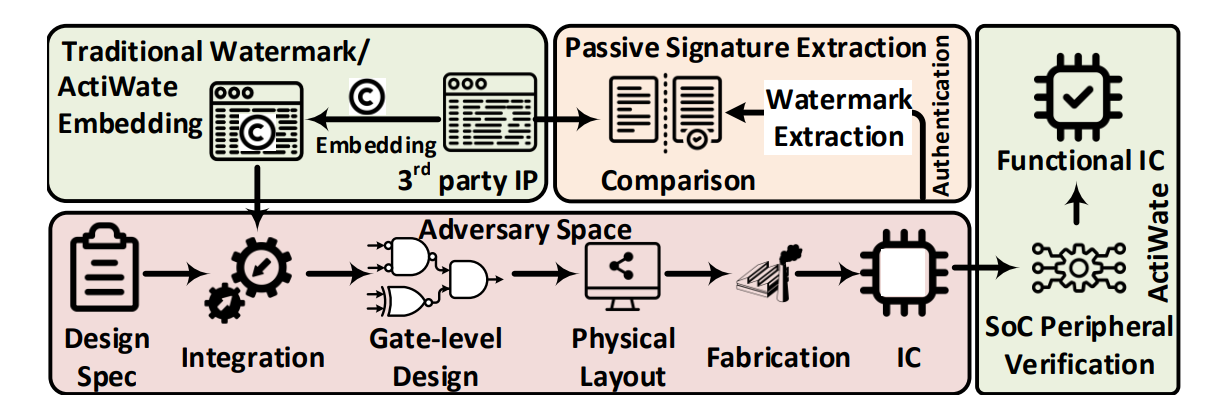
\includegraphics[width=\columnwidth]{fig1.png}
	\caption{SoC design flow using third-party IPs (red box), along with the
		watermark/\textit{ActiWate} embedding (green box) and signature extraction flow
		(orange box). \textit{ActiWate} does not require any post-silicon signature extraction,
		rather it relies on active verification of the SoC peripherals (green box).}
	\label{fig1}
\end{figure}

The rest of the paper is organized as follows- Section \ref{sec2} provides
a threat model for the active IP watermarking, existing FSM-based
watermarking techniques, and their pitfalls. Section \ref{sec3} presents the
detailed overview of \textit{ActiWate}, watermarking process of peripheral
verification. Section \ref{sec4} shows how \textit{ActiWate} performs system and
IP agnostic verification using the peripheral-based associated CRPs
in different RISC-V and ARM SoCs. Section \ref{sec5} discusses the PPA
overhead analysis of the watermarked IPs and discusses the resiliency
against possible attacks. Section \ref{sec4} concludes the paper.


\section{BACKGROUND AND MOTIVATION}
\label{sec2}
\subsection{\textit{Threat Model}}
\label{sec2a}
A watermark identifies IP piracy/overuse by marking an asset with
a known signature. In hardware design flow, watermarking is the
process of embedding a signature (or a unique function) within the
IP core without affecting the original functionality of the design as
shown in Fig. 1. The watermark signature can be used to authenticate
IP ownership. Watermarking has always been a passive method
that does not prevent IP infringement, piracy, or overproduction of
integrated circuits but can detect IP reuse. A watermarking solution
should possess the following features \cite{Anandakumar2022}:

\begin{enumerate}[label=(R\arabic*)]
	\item \underline{Fidelity}: The watermark should not interfere with the original IP functionality or specified/expected IP performance.
	
	\item \underline{Uniqueness}: The watermark signature should be unique to each IP core to eliminate any chance of collision.
	
	\item \underline{Resiliency}: Watermarks for authenticating IPs in an SoC are susceptible to noise from the neighboring IPs. Hence, the watermark should be resilient to the interference from neighboring IPs.
	
	\item \underline{Non-redundancy \& robustness}: The watermark should be properly incorporated with IP functionality to eliminate any chance of illegal identification, removal, or modification.
	
	\item \underline{Efficiency}: The watermark should be easy to verify with a minimum implementation overhead and low observability.\\
\end{enumerate}
  
 Fig. \ref{fig1} shows IP watermark embedding, conventional semiconduc
tor design flow, and watermark signature extraction-based authenti
cation process. Unlike the existing watermarking techniques, in this
paper, we consider any parties in the semiconductor supply chain
(i.e., SoC integrators, design service providers, offshore foundries,
and test facilities) in the adversary space (red box in Fig. \ref{fig1}).
While traditional watermarking techniques rely on a passive signature
extraction process \cite{Kibria2022_RTL}, \textit{ActiWate} deploys a signature-less automated
verification of the peripheral IPs to block IP functioning in an
illegitimate SoC actively.

\subsection{\textit{Existing Watermarking and their Pitfalls}}
\label{sec2b}
 Several watermarking approaches have been described in the
literature for IP authentication. These watermarking approaches can
be roughly classified into five groups: (1) Constraint-based water
marking, (2) Digital signal processing (DSP)-based watermarking, (3)
Finite state machine (FSM)-based watermarking, (4) Test structure
based watermarking and (5) Side channel-based watermarking.

Constraint-based watermarking relies on a complex optimization
problem. In this optimization problem, finding an appropriate solution
or enumerating enough acceptable solutions grows exponentially with
input size. A set of embedded constraints is first generated from
the encrypted authorship message. The embedded constraints are
blended with the cover constraints, derived from the original design
specifications, to generate the stego constraints. EDA tools are then
used to find a near-optimal solution to the stego problem. As a result,
a watermarked IP core will satisfy both the original and embedded
constraints \cite{Tehranipoor2011}-\cite{Hong1998}. In DSP-based watermarking techniques, design
ers adjust filters’ decibel (dB) requirements to embed watermark
signatures without compromising their performance. In this case, the
watermark signature is a single character (7 bits) encoded into a
high-level digital filter \cite{Chapman2000},\cite{Rashid1999}. FSM-based watermarking techniques
modify the State Transition Graph (STG) of an FSM to embed a
watermark into the circuit. Depending on the watermarking strategy,
FSM-based watermarking methods can be classified into two types:
state-based and transition-based. New states or encodings are added
in state-based watermarking schemes. \cite{Oliveira2001},\cite{Lewandowski2012}. In contrast, transition
based watermarking techniques use previously unused transitions or
add new ones \cite{Torunoglu2000}-\cite{Cui2011}. For the FSM-based watermarking approach,
authorship proof is verified by observing output responses that follow
specific input patterns. Testing-based watermarking techniques embed
a watermark into a test sequence at the behavioral level. Test signals
of an IP must be traceable after IPs are integrated into full SOCs. Test
based watermarking techniques \cite{Cui2015} take advantage of this fact to
combine the test sequence with the circuit for generating a watermark.
During test mode, the selected IP sends out output test patterns and
watermark sequences. For side-channel-based watermarking, the side
channels of a circuit is engineered to contain a watermark. In \cite{Ziener2006}-\cite{Marchand2014},
power signature-based watermarking techniques were introduced for
protecting IP cores which relies on the measurement of the power
consumption for watermark verification.

For constraint-based watermarking, watermarked IPs cannot be
authenticated in the field without opening their encapsulation. In addi
tion to being expensive, extracting the hidden watermark destroys the
working IC. The DSP-based and side-channel-based watermarking
techniques are susceptible to design variations and noise \cite{Anandakumar2022}. FSM
based watermarking is usually based on the observed bit sequences at
the output. However, once the watermarked IP is integrated into the
chip, the outputs of the FSM cannot be observed externally. Although
testing-based watermarking techniques allow external observability,
they are susceptible to scan chain modifications. Thus, all of these
watermarking techniques fail to meet the requirements II-A. Also,
these watermarking techniques are not active in nature (for IP
protection) and thus cannot prevent IP piracy.

\section{METHODOLOGY}
\label{sec3}
\subsection{\textit{Overview}}
\label{sec3a}
Developing the active watermarking implementation begins with a
thorough understanding of how to protect an IP from a rogue SoC
integrator and what tools are at our disposal to formulate an effective
technique. \textit{ActiWate} is an IP-level FSM watermarking verification
where the watermarked IP conducts communication with other SoC
peripherals so that it can confirm it is in the correct SoC. To follow
this plan, we built on the requirements listed in section \ref{sec2a} with
additional ones to constrain our methodology:

\begin{enumerate}[label=(R\arabic*)]
	\setcounter{enumi}{4}
	\item \underline{IP Usability}: The IP cannot enter a functional mode if the
	watermark verification fails.
	\begin{figure}[H]
		\centering
		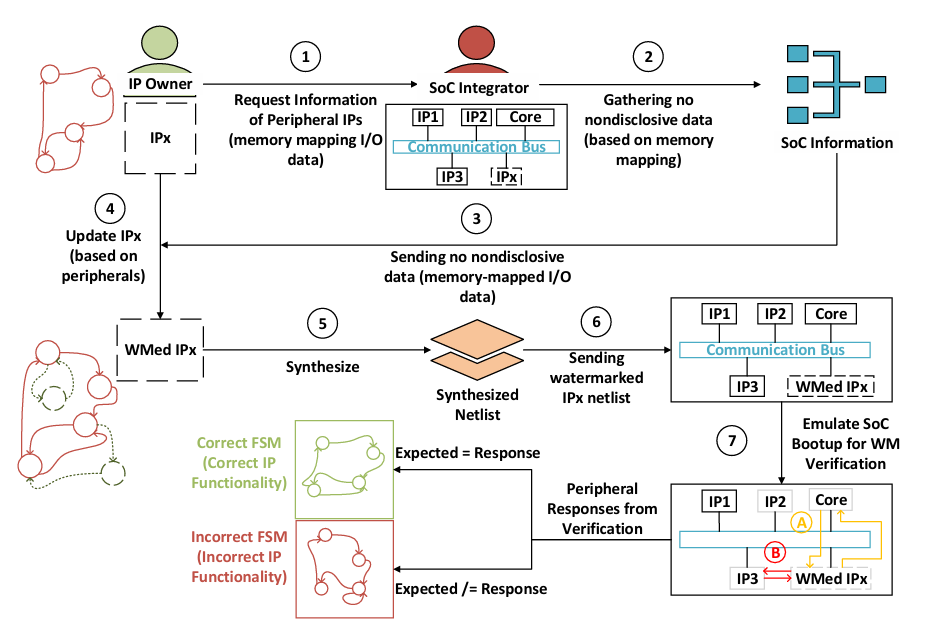
\includegraphics[width=0.5\textwidth]{fig2.png}
		\caption{\textit{ActiWate} Verification Process Framework}
		\captionsetup{justification=centering}
		\label{fig2}
	\end{figure}
	
	\item \underline{SoC Agnostic}: The watermark protocol cannot rely on specific
	SoC architectures for verifying that the IP is in the correct SoC.
	
	\item \underline{Bus Communication}: Communicating between the IP and the
	SoC peripherals can only be done with the available SoC
	communication bus architecture.
	
	\item \underline{Integrated FSM}: IP functionality and the watermark verification
	are integrated together into a single FSM where watermark
	removal results in a loss of functionality.\\
\end{enumerate}

Taking these new requirements, we can further elaborate the
methodology. The peripherals are communicated with via a pinging
system consisting of addresses and request prompts unique to the
watermark verification. Once the watermarked IP receives the correct
responses to the requests sent to the peripherals, then the verification
confirms that the IP in the correct SoC and renders the IP usable. If at
any point during the verification that an incorrect result is sent back to
the watermarked IP as the response in a CRP, then the IP enters a state
in which it does not function correctly. Although the methodology
breaches R1 in section \ref{sec2a}, the IP functionality is unchanged if the
verification succeeds. If it does not, the original IP functionality is
still present within the IP; however, the verification failure results
in the IP entering a different mode of operation where it functions
incorrectly. This will be further explained in section \ref{sec3b}. It should
also be mentioned that we do not need to observe the outputs of
the FSM, a pitfall mentioned in section \ref{sec2b}, because the \textit{ActiWate}
process does not need FSM outputs to be verified externally.

\subsection{\textit{Process}}
\label{sec3b}
The \textit{ActiWate} process begins with a communication between the
IP owner and the SoC integrator. As seen in Fig. \ref{fig2}, the IP owner first
requests information from the SoC integrator about the peripherals
and the physical mapping addresses within the SoC. It is important
to note that despite our threat model, the SoC integrator can see
the IP owner as a threat because of this request for information
about peripheral functionality and address spaces. Therefore, the
SoC integrator will send this information to the IP owner, but
the information will undergo garbling to enable a two-party secure
computation \cite{Hashemi2022}. As for the functionality aspect for the IP owner,
despite receiving information about a specific SoC, the watermark
protocol is SoC agnostic. After the IP owner receives this information,
a number of peripherals are chosen at random to act as the points
of communication for the watermark verification. Even though the
peripherals are chosen at random, there is a time constraint the IP
owner should follow to make the verification happen swiftly and
efficiently. The IP owner then sends the synthesized netlist with the

\begin{figure}[H]
	\centering
	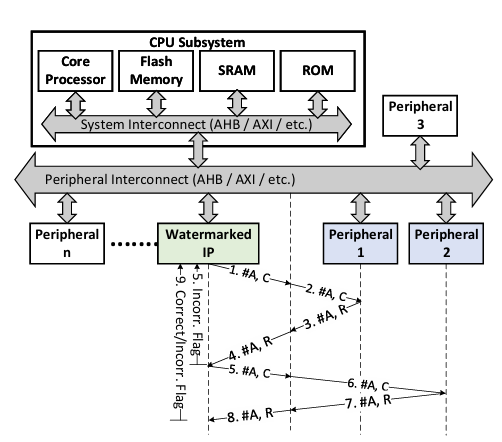
\includegraphics[width=0.5\columnwidth]{fig3.png}
	\caption{ \textit{ActiWate} Pinging Verification Steps within the Watermarked IP FSM.
		The watermarked IP (breen box) sends challenge (C) to and expects response
		(R) from the peripheral IPs (blue box) based on their given address (A) that
		it receives from the SoC integrator.}
	\captionsetup{justification=centering}
	\label{fig3}
\end{figure}

integrated watermark verification to the SoC integrator. After the
watermarked IP is placed within the SoC, the SoC goes through its
own simulation that emulates the bootup process, which starts the
watermark verification.

The verification follows a series of steps by which the watermarked
IP communicates with the SoC peripherals, and the steps can be seen
in Fig. \ref{fig3}. First, the watermarked IP starts the verification with the
FSM as it sets up a challenge prompt to the first peripheral consisting
of the input signals and the memory address space for the peripheral’s
data registers. It is important to note that the addresses used in
verification are unique and limited to the watermarking protocol. The
addresses are secret, but they exist within the defined address spaces
of the SoC. The request is then sent via the SoC communication
bus. After receiving the prompt, the peripheral calculates a response
using its preexisting functionality and sends a response back to
the watermarked IP via the communication bus. This exchange is
denoted by A in step 7 in Fig. \ref{fig2} and seen in further detail in
Fig. \ref{fig3}. Upon receiving the response, the watermarked IP checks
it with the expected value to the prompt. If the response matches
the expected value calculated by the developer, the verification
continues to the next peripheral, which follows the same steps as
with the first peripheral. It is important to mention that there is
no additional circuitry to calculate the expected response as that
would incur high overhead; these values are simply set based on
the functionality and specific inputs to the peripheral. For testing
purposes, we relied on the verification of two peripherals as seen in
section \ref{sec4}. Once, the response from the last peripheral is confirmed
with the expected value, the watermarked IP ends the verification and
enters the functional mode. If at any point the verification fails, then
the IP will discontinue the verification and enter a mode where it
functions incorrectly.

To elaborate on each state of the protocol, the \textit{ActiWate} process
depends first on an initial collaboration between the IP owner and the
SoC integrator as seen in steps 1-4 in Fig. \ref{fig2}. This is a necessary step
because the IP owner needs to understand the available peripherals in
the SoC and their functionality to develop a verification depends on
the communication between the IP and those peripherals. Moreover,
this step can act as the initial vetting process against an attacker.

To state again, the threat that the \textit{ActiWate} process is meant to act
against is a rogue SoC integrator. If the SoC integrator refuses to
give the IP owner information regarding the peripherals within the
SoC, this could mean that this is a rogue SoC integrator that does not
want to share the addresses as well as CRPs to the IP owner. If the
SoC integrator complies with the request for information from the IP
owner, the integration of the watermark verification can proceed.

To make this process active, the \textit{ActiWate} watermark protocol is
automated such that when the SoC begins its own simulation, the
watermarked IP begins its verification to figure out if it is placed
in the correct SoC or not. This is done by integrating the watermark
verification into the functional FSM of the IP. No manual intervention
is necessary. How the watermark is integrated into the FSM can
be described as a form of activating the IP’s functionality. When
the verification succeeds for the first peripheral, half of the IP’s
functionality is made available. This can be thought of as part of
the calculation towards the result of the IP is done after the initial
part of the verification is done.

At the most basic terms, the verification is a communication
protocol between the watermarked IP and neighboring peripherals
in an SoC. To establish this communication, we used the SoC
communication bus architectures. The communication bus sends and
receives data from all peripherals that make up the SoC. For the
\textit{ActiWate} implementation, the watermarked IP is set up as a master
in the communication protocol so that it can send requests for data to
the slave peripherals. As stated earlier, \textit{ActiWate} is SoC agnostic, but
the process needs to be tailored to the communication protocol that
exists in a SoC. However, the process is also bus agnostic, meaning
that any communication protocol is applicable to the verification.

The secure IP uses the communication protocol to send a request
for data to the SoC peripherals that are a part of the verification
process. Within the request, there is an unique address and the request
itself. The address is an important part of the request because it
is necessary for the communication bus so that the data reaches
the correct peripheral. If the address of the request does not match
that of a neighboring peripheral, the verification fails, and the IP
is rendered functionally incorrect. If the address matches, then the
request goes through. However, a simple acknowledgement is not
enough because the peripheral must match in functionality as well.
Then, the response is sent back through the communication bus to
the watermarked IP so that it can be matched to the expected value.
To make the implementation more thorough, we rely on the response
of more than one neighboring peripheral where after the verification
succeeds for one peripheral, the following peripheral’s verification is
triggered. Once all pass the verification, the watermarked IP has fully
confirmed its location in the golden SoC.

If the verification succeeds, the secure IP functions correctly within
the SoC. If not, then the IP functions incorrectly. We chose to have
the IP give incorrect responses rather than shutting off because there
is a lower chance of the attacker realizing that there is a verification
process put into the IP. The rogue SoC integrator then cannot utilize
the correct functionality of the IP, and the value of the insecure SoC
drops in the market since there is incorrect functionality present.

\section{CASE STUDIES}
\label{sec4}
The \textit{ActiWate} watermark verification was developed on three
different SoC’s that differ from each other in complexity as well
as architecture. We implemented ActiWate on the following Soc
benchmarks.

\begin{enumerate}
	\item Ultraembedded SoC \cite{RISC-V2024}: RISC-V Test SoC with an AXI4 bus
	architecture
	
	\begin{table}[h!]
		\centering
		\caption{ Configuration of nine different situations created to demonstrate
			the robustness of \textit{ActiWate}. We utilized Adder and AES as watermarked IP
			(W.IP) and ALU, RSA, AES, and Decoder as peripheral IP for verification.}
		\captionsetup{position=above}
		\label{t1}
		\begin{tabular}{c c c c c c c} 
			\hline
			\underline{SoC} & \multicolumn{2}{c}{\underline{Situation 1, 4, 7}} & \multicolumn{2}{c}{\underline{Situation 2, 5, 8}} & \multicolumn{2}{c}{\underline{Situation 3, 6, 9}} \\ 
			& \underline{W.IP} & \underline{Peripherals} & \underline{W.IP} & \underline{Peripherals} & \underline{W.IP} & \underline{Peripherals} \\ 
			Ultra SoC & Adder & \{ALU, RSA\} & Adder & \{AES, Dec.\} & AES & \{ALU, Dec.\} \\ 
			ARM SoC & Adder & \{ALU, RSA\} & Adder & \{AES, Dec.\} & AES & \{ALU, Dec.\} \\ 
			CVA6 SoC & Adder & \{ALU, RSA\} & Adder & \{AES, Dec.\} & AES & \{ALU, Dec.\} \\ 
			\hline
		\end{tabular}
		

	\end{table}
			
	\item ARM SoC \cite{or1200_soc}: ARM-based SoC with an AHB-lite bus archi
	tecture
	
	\item CVA6 RISC-V CPU Soc \cite{CVA62024}: 6-stage RISC-V SoC with an
	AXI4 bus architecture \\
\end{enumerate}

For all three benchmarks, three situations were applied to see the
results of differing implementations. The descriptions of the situations
are as follows:

\begin{enumerate}
	\item ALU and RSA Peripherals: For a watermarked adder IP, ALU
	and RSA are the peripherals chosen for the \textit{ActiWate} verification.
	\item AES and Decoder Peripherals: For a watermarked adder IP, AES
	and a decoder are the peripherals chosen for verification.
	\item Watermarked AES: For a watermarked AES IP, ALU and a
	decoder are the peripherals chosen for verification.\\
\end{enumerate}

The situations with the corresponding SoC are listed in Table \ref{t1}.
\subsection{ALU \& RSA \textit{Peripherals}} 
\label{sec4a}

Situations 1, 4, and 7 in Table \ref{t1} cover the usage of the \textit{ActiWate}
process integrated into an adder IP with the chosen peripherals ALU
and RSA. For the secure IP, the functionality is basic, with two
inputs (in1, in2) and one output. However, it can still be divided into
parts such that the watermark process can activate each part of the
functionality as the verification progresses. The process begins with
the secure IP pinging the ALU for a response to a set of three inputs
(control, input1, input2). The three inputs have their own memorymapped addresses used for the bus protocol, and the inputs are sent to
the ALU peripheral’s data registers. For Situation 4, the bus protocol
is different from Situations 1 and 7 since it is an AHB-lite bus. This
bus architecture accommodates only one master. In this situation,
the IP owner must communicate with the SoC integrator that an
AHB interconnect matrix must be placed in an IP other than the
watermarked core. For testing purposes, we included the AHB matrix
so that the adder IP can act as a master in the bus protocol.
Upon arrival, the ALU calculates the response to the ping with
its normal functionality and sends the response back through the
communication bus to the secure IP. If the response matches the
expected, then in1 is moved into a data register. Then, the secure IP
pings the RSA for a response to a set of inputs (p,q: prime numbers,
encrypt decrypt: enable, msg in: input, and msg out: output). Again,
this information is sent through the communication bus, with each
input having a unique address. The same steps occur with the RSA
calculating a response to the ping and sending the response back to
the secure IP, which then checks the response with the expected. If
this verification succeeds, then in2 is moved to a data register. The
movement to the data registers is how an IP with a small amount
of functionality can be unlocked with the \textit{ActiWate} process because
the adder computes the response using the data registers with the
input values rather than the inputs to the IP itself. Once both data
registers have been filled with the input values, the correct response
is calculated, showing that the IP is functioning normally.

\subsection{AES \& Decoder peripherals}
\label{sec4b}
For situations 2, 5, and 8 in Table \ref{t1}, we followed a similar template
of subsection \ref{sec4a} and integrated \textit{ActiWate} into the same adder IP
\begin{table}[h!]
	\centering
	\caption{Power (PO), and area (AO) overhead of \textit{ActiWate} across different
		situations defined in Table \ref{t1}. Please note that \textit{ActiWate} does not incur any
		performance overhead other than initial latency for verification}
	\label{t2}
	\begin{tabular}{lcc cc cc}
		\hline
		\underline{SoC} & \multicolumn{2}{c}{\underline{Situation 1,4,7}} & \multicolumn{2}{c}{\underline{Situation 2,5,8}} & \multicolumn{2}{c}{\underline{Situation 3,6,9}} \\
		&\underline{AO(\%)} & \underline{PO(\%)} & \underline{AO(\%)} & \underline{PO(\%)} & \underline{AO(\%)} & \underline{PO(\%)} \\
		Ultra SoC & 21.15\% & 24.07\% & 23.54\% & 26.22\% & 2.49\% & 3.13\% \\
		ARM SoC   & 19.89\% & 21.28\% & 25.55\% & 26.91\% & 2.53\% & 3.07\% \\
		CVA6 SoC  & 20.71\% & 22.72\% & 23.89\% & 24.78\% & 2.64\% & 3.19\% \\ \hline
	\end{tabular}
	
\end{table}
except with two other peripherals, AES and a decoder. A decoder
IP was used primarily to show that the verification process can use
peripherals with simple functionality. Therefore, the process does not
restrict itself to peripherals with complex functionality. Following the
same process as in subsection \ref{sec4a}, the watermarked IP pings the
AES peripheral with the necessary inputs (cs,we: enables, address,
and write data) and the associated unique addresses to calculate a
response. If the AES response matches the expected value, then the
value of in1 is moved into a data register. Then, the verification moves
to ping the 2-to-4 decoder, consisting of the inputs (a, b: inputs, en:
enable) for a response. The response is sent back through the bus to
the secure IP, and if the response matches the expected, the value in2
is loaded into a data register. The secure IP enters functional mode
after the full verification succeeds.

\subsection{\textit{Watermarked AES IP}}
\label{sec4c}
We created the last category of situations to prove the robustness
of \textit{ActiWate} watermark by integrating an IP with more complex
functionality. We implemented the watermark into a cryptographic
module, AES. Using the decoder and ALU peripherals, the same
pinging system and subsequent verification checks are done for
situations 3, 6, and 9 from Tabel \ref{t1}; however, the activation of
functionality for the secure IP differs. Within the AES functional flow,
three nested \textit{if} statements depend on three of the inputs. Therefore,
the IP unlocking is as follows: the message to be encrypted and the
address for functionality is loaded into data registers after the first
peripheral passes the verification, and the two enables are loaded
into data registers after the second peripheral passes the verification.
Once those values are loaded, the value for the encrypted response
is calculated since the data registers change triggers the function’s
sensitivity list.

\section{RESULTS AND ANALYSIS}
\label{sec5}
 In Section \ref{sec4} we created nine different SoC scenario based on the
configuration presented in Table \ref{t1} and demonstrated the robust active
watermarking flow enabled by ActiWate. In this section we present
the power, performance, and area overhead of ActiWate in a practical
SoC scenario and analyze its security.
\subsection{\textit{Overhead Analysis}}
\label{sec5a}
To experimentally evaluate the practical applicability of \textit{ActiWate},
we implemented all the different SoC scenarios presented in Table \ref{t1}.
We implemented \textit{ActiWate} in the target IP and integrated it with the
rest peripherals of the SoC. Later, we utilized Synopsys Design
Compiler to synthesize the integrated SoC using Synopsys
32nm academic library. We collected the total power and area
consumed by \textit{ActiWate} and reported the overhead in Table \ref{t2} by
comparing it with the baseline. Please note from Section \ref{sec3} that
\textit{ActiWate} does not interfere with the original functionality of the IP or
the SoC it is integrated with; rather, it initiates a series of verification
protocols that validates the presence of the IP in the intended SoC
irrespective of the design or architecture. Therefore, \textit{ActiWate} does
not incur any performance overhead. Due to additional verification  that takes place before the IP starts functioning regularly, the IP
incurs initial latency. However, once the IP is verified successfully
by \textit{ActiWate}, it functions as expected, and there is no impact on the
throughput. In terms of the power and area overhead induced by
\textit{ActiWate}, please not from Table \ref{t1} that the situation \{1, 4, 7\} and \{2, 5, 8\} targets same IP (adder) for watermarking. Hence, the power
and area overhead for these six situations are very similar. The size
of \textit{ActiWate} does not depend on the host IP. Hence, the power and
area overhead is bit more for adder in situation \{1, 2, 4, 5, 7, 8\} than
for a reasonable size IP, e.g., AES in situation \{3, 6, 9\} in Table \ref{t2}.

\subsection{Security Analysis}
\label{sec5b}
When protective circuitry is placed into an IP, there are several
ways to bypass the security or remove the protection altogether.
Moreover, an attacker can observe an IP with thorough analysis
to take advantage of holes in the security. The security analysis
for \textit{ActiWate} emphasizes possible attacks against watermarks by
performing removal and forgery attacks as well as attacks that target
specific features of \textit{ActiWate}, e.g., address collision and bus spoofing
attacks.

\begin{enumerate}
	\item \textit{ Removal Attacks}: When a watermark is integrated into an
	IP, there exists the threat of removing or bypassing the watermark
	circuitry to dismantle the copyright proof mechanism of the secure
	IP \cite{Yasin2020}. If a removal attack is successful, the IP no longer carries any
	proof of authorship. For the \textit{ActiWate} process, it is important to note
	that the watermark FSM and the functional FSM are tightly integrated
	together. Moreover, in \textit{ActiWate}, IP is shared with the SoC integrator
	in the form of synthesized netlist to hide watermark circuitry and
	peripheral (that are utilized for verification by the watermarked IP)
	addresses from the rogue SoC integrator. Additionally, one of the
	key features that is indicative of this is the fact that the secure IP
	functionality needs to be activated by the steps of the watermark
	verification. Without the verification, the IP is rendered unusable.
	Therefore, even if an attacker steals the IP and can successfully
	remove the watermark circuitry, the IP cannot be made functional.
	
	\item \textit{Forgery Attacks}: Consider another scenario if the watermarked
	IP is stolen from the contracted SoC integrator. A forgery attack is
	then performed by which the attacker inserts his own watermark in
	the original owner’s watermarked IP \cite{Karmakar2022}. In this scenario, there can
	be two possibilities for the attacker to pirate the IP. The first is that
	the attacker can remove the existing watermark and replace it with
	his forged watermark. As discussed in section \ref{sec5b}, it is extremely
	difficult to remove \textit{ActiWate} from the IP without compromising the
	IP functionality because of its close coupling with the original IP.
	Therefore, the second possibility for the attacker is to insert the forged
	watermark on top of the existing watermark. However, \textit{ActiWate} will
	fail its verification in an SoC that does not contain the required IP
	for verification, and the IP will not be functional regardless of the
	forged watermark passing its own verification.
	
	\item \textit{Address Collision or Tampering}: An important part to the
	\textit{ActiWate} methodology is the utilization of the communication bus,
	which works with the SoC peripherals by communicating through
	their address spaces. If the watermarked IP is stolen and then
	integrated with an illegitimate SoC, there exists a chance that the
	address space mapped to a peripheral necessary for watermark
	verification matches the address space of a peripheral within the
	rogue SoC. This is defined as an address collision in the sense that
	the verification peripheral’s address space overlaps that of the rogue
	SoC’s peripheral \cite{Harsh2008}. If the \textit{ActiWate} methodology relied solely on
	pinging address spaces without any CRP, then the secure IP would
	be verified successfully within a rogue SoC. However, this is not the case with ActiWate because our method relies on pinging the
	address space as well as collecting the responses of the challenges
	sent from the watermarked IP. The probability of both the address
	space and functionality matching between the peripheral of the trusted
	SoC and the peripheral of an untrusted SoC is extremely low. It also
	needs to be considered that more than one peripheral is necessary
	for verification making the probability decreases even further. Equ. 1
	considers the probability of address space and functionality overlap of
	two peripherals within the rogue SoC. The probability of the address
	space matching for each peripheral is $2^n$ where n is the size of the
	address space in bits. Then, to consider the functionality matching,
	we use $\alpha$ and $\beta$ for peripheral A and peripheral B respectively.
	
	\begin{equation}
		p \approx \alpha \times 2^n \times \beta \times 2^n\\
	\end{equation}
	
	 The overall probability is extremely small, even for just consid
	ering one peripheral. If more than one peripheral is considered, the
	probability gets smaller once multiplied per peripheral.
	
	\item  \textit{Bus Spoofing Attacks}: Because the \textit{ActiWate} implementation
	relies heavily on the usage of the SoC bus architecture, there is a high
	risk of bus spoofing attacks carried out by the rogue SoC integrator.
	The transmission of the ping to the peripheral from the secure IP and
	the subsequent response back to the secure IP can be compromised if
	either transmission is monitored or probed by the untrusted party \cite{Iehira2018}.
	To secure \textit{ActiWate} against the SoC bus spoofing attacks, we deploy
	constant obfuscation \cite{Bakken2004} of the transmissions and the address spaces
	used in the verification process. The constant obfuscation changes all
	the data points in the same way, whether absolute or relative. This
	approach minimizes observable data from the secure IP. Hence, it is
	difficult to conduct a bus spoofing attack if the IP is stolen.
\end{enumerate}

\section{CONCLUSION}
\label{sec6}
 \textit{ActiWate} is an IP-level active watermarking scheme to probe the
authorship of an IP against a rogue SoC integrator, a threat often
ignored in talks about IP piracy. Existing watermark techniques do
not prevent IP theft and, therefore, are passive in nature. Moreover,
specific watermark techniques have constrained approaches that pre
vent ease in verification. \textit{ActiWate} is a completely novel solution to
verification issues regarding proof of IP authorship. Our methodology
satisfies the requirements of a watermark and has a unique approach
to verification where the FSM within the secure IP ensures an
automated watermarking protocol whereby the IP knows whether
or not it is in the correct SoC. To test out the methodology, we
implemented \textit{ActiWate} in three different SoCs with a variety of test
cases covering how the watermarking protocol works. As for the
efficiency of our watermarking scheme, we conducted an overhead
analysis where each SoC is checked for how much of an overhead
difference the watermark causes. Furthermore, the security analysis
is conducted by understanding the types of attacks our protocol
is susceptible to and what measures we have in place to prevent
these kinds of attacks. Overall, \textit{ActiWate} acts as a new approach to
watermarking with its unique automated methodology that can protect
an IP against a less talked about the threat, the SoC integrator.



\section*{ACKNOWLEDGEMENT}
This work was supported by the Synopsys and DARPA AISS Grant
\#HR0011-20-9-0043.

\bibliographystyle{plain}
\bibliography{references} 
\end{document}
